\documentclass[12pt,english, openany]{book}
%%%%%%%%%%%%%%%%%%%%%%%%%%%%%% Loading packages that alter the style
\usepackage[]{graphicx}
\usepackage[]{color}
\usepackage{alltt}
\usepackage[T1]{fontenc}
\usepackage[utf8]{inputenc}
\usepackage{multicol}
\usepackage{amsmath}
\usepackage{stmaryrd}
\usepackage{booktabs}
\usepackage{calc}
\usepackage{amsmath, amssymb}
\usepackage{bbold}
\usepackage[ruled,lined]{algorithm2e}
\usepackage{tikz}
\usepackage{cite}
\usepackage{svg}
\usepackage{lmodern}
\usepackage{minted}

\setcounter{secnumdepth}{3}
\setcounter{tocdepth}{3}
\setlength{\parskip}{\smallskipamount}
\setlength{\parindent}{0pt}
\DeclareUnicodeCharacter{0301}{\'{ }}

% Package for figures
\usepackage{subfigure, float}

% Set page margins
\usepackage[top=100pt,bottom=100pt,left=68pt,right=66pt]{geometry}

% Package used for placeholder text
\usepackage{lipsum}

% Prevents LaTeX from filling out a page to the bottom
\raggedbottom

% Adding both languages
\usepackage[english, french]{babel}

% All page numbers positioned at the bottom of the page
\usepackage{fancyhdr}
\fancyhf{} % clear all header and footers
\fancyfoot[C]{\thepage}
\renewcommand{\headrulewidth}{0pt} % remove the header rule
\pagestyle{fancy}

% Changes the style of chapter headings
\usepackage{titlesec}
\titleformat{\chapter}
   {\normalfont\LARGE\bfseries}{\thechapter.}{1em}{}
% Change distance between chapter header and text
\titlespacing{\chapter}{0pt}{-10pt}{1\baselineskip}

% Adds table captions above the table per default
\usepackage{float}
\floatstyle{plaintop}
\restylefloat{table}

% Adds space between caption and table
\usepackage[tableposition=top]{caption}

% Adds hyperlinks to references and ToC
\usepackage{hyperref}
\hypersetup{hidelinks,linkcolor = black} % Changes the link color to black and hides the hideous red border that usually is created

% If multiple images are to be added, a folder (path) with all the images can be added here 
\graphicspath{ {images/} }

% Separates the first part of the report/thesis in Roman numerals
\frontmatter

\usepackage[nottoc, notlof, notlot]{tocbibind}

\bibliographystyle{plain}

%% Settings for the pseudocode
\SetKwFor{Tq}{tant que}{faire}{fin tq}%
\SetKwIF{Si}{SinonSi}{Sinon}{si}{alors}{sinon si}{sinon}{fin si}%
%%%%%%%%%%%%%%%%%%%%%%%%%%%%%% Starts the document
\begin{document}

%%% Selects the language to be used for the first couple of pages
\selectlanguage{french}


%%%%% Adds the title page
\begin{titlepage}
	\clearpage\thispagestyle{empty}
	\centering
	\vspace{1cm}

	% Titles
	% Information about the University
	{\normalsize UTC \\ 
		PROJET TX 2024}
 \\
		
		\vspace{3cm}
	{\Huge \textbf{A guinea pig for deep learning with many classes}} \\

	\vspace{3cm}
	{\normalsize Deseure--Charron Alexis \\ Calzas Vincent \\ \par}
	\vspace{0.7cm}
 
    { \textbf{Référent école}} \\
    {Yves Grandvalet}
    \vspace{4.5cm}

    
    \centering 
    
\includegraphics[scale=0.07]{images/UTC-SU.jpg}

	\pagebreak

\end{titlepage}

\tableofcontents{}

\newcommand{\hiddensubsection}[1]{
    \stepcounter{subsection}
    \subsection*{\hspace{1em}{#1}}
}

\mainmatter

\chapter{Introduction}

En Deep Learning, les problèmes de classification peuvent composer plusieurs centaines voire plusieurs milliers de classes. Balestriero a montré en 2022 \cite{NEURIPS2022_f73c0453} que les effets de la régularisation et de l'augmentation de données dépendent des classes du problème, ce qui signifie que la valeur optimale de l'hyper-paramètre de régularisation (exemple : le weight decay) peut varier pour chacune des classes. L'hyper-paramètre est alors choisi en faisant un compromis entre les différentes classes en étant ainsi optimal pour aucune classe. \\

L'objectif de notre projet est alors d'étudier l'impact de l'ajustement de la dernière couche d'un modèle de classification en gelant les poids des couches précédentes déjà pré-entraînés. Pour cela, nous utiliserons un ResNet50 entraîné sur ImageNet afin de récupérer les sorties de l'avant-dernière couche et ainsi, à partir de ces résultats, ajuster l'entraînement d'un modèle de régression logistique correspondant à la dernière couche du modèle initial, pour étudier l'impact des régularisations.

\chapter{Etat de l'art}
\section{Classification par des réseaux de neurones à convolution}
\subsection{Concept}

\subsubsection{Réseau de neurones (Perceptron multicouches)}
\label{subsubsec:ANN}

\def\layersep{2.5cm}
\begin{figure}[h]
    \centering
    \begin{tikzpicture}[shorten >=1pt,->,draw=black!50, node distance=\layersep]
        \tikzstyle{every pin edge}=[<-,shorten <=1pt]
        \tikzstyle{neuron}=[circle,fill=black!25,minimum size=17pt,inner sep=0pt]
        \tikzstyle{input neuron}=[neuron, fill=blue!50];
        \tikzstyle{output neuron}=[neuron, fill=purple!50];
        \tikzstyle{hidden neuron}=[neuron, fill=pink];
        \tikzstyle{annot} = [text width=4em, text centered]
        \foreach \name / \y in {1,...,4}
            \node[input neuron, pin=left:Input \y] (I-\name) at (0,-\y) {};
        \foreach \name / \y in {0,...,5}
                \path[yshift=0cm]
                    node[hidden neuron] (A-\name) at (\layersep,-\y cm) {};
        \foreach \name / \y in {0,...,5}
                \path[yshift=0cm]
                    node[hidden neuron] (B-\name) at (2*\layersep,-\y cm) {};
        \node[output neuron, pin={[pin edge={->}]right:Output}] (O) at (\layersep+\layersep+\layersep, -2.5) {};
            \foreach \source in {1,...,4}
            \foreach \dest in {0,...,5}
                \path (I-\source) edge (A-\dest);
                \foreach \source in {0,...,5}
                \foreach \dest in {0,...,5}
                    \path (A-\source) edge (B-\dest);
            \foreach \source in {0,...,5}
                \path (B-\source) edge (O);
        
        \node[annot, above of=A-0, node distance=1cm] (hl1) {Hidden layer 1};
        \node[annot, left of=hl1] {Input layer};
        \node[annot, right of=hl1] (hl2) {Hidden layer 2};
        \node[annot, right of=hl2] {Output layer};
    \end{tikzpicture}
    \caption{Représentation schématique d'un réseau de neurones artificiels}
    \label{fig:ann}
\end{figure}

Un réseau de neurones est un système composé d'une multitude de neurones disséminés sur plusieurs couches connectées entre-elles. Pour le problème de classification, le réseau renvoie en sortie une probabilité pour chaque classe en fonction de l'image mise en entrée. \\

Au sein d'une couche, chaque neurone reçoit en entrée les sorties de la couche précédente. Puis le neurone calcule une combinaison linéaire des données en entrée avec des coefficients appelés poids. Ce résultat passe ensuite dans une fonction d'activation avant d'être délivré en sortie.\\

La dernière couche délivre les probabilités associés à chaque classe en utilisant une fonction d'activation. Dans notre cas multi-classe : softmax.\\

Pour obtenir l'erreur de classification, on calcule une fonction de coût (loss). Les poids introduits précédemment sont ajustés par rétropropagation du gradient. En partant de la fin, on calcule pour chaque couche les poids qui minimisent la fonction de perte.\\



\subsubsection{Les caractéristiques}
Les caractéristiques (features en anglais) sont des représentations de "zones intéressantes de l'image" comme des points, des zones ou des régions. Pour être plus précis, les caractéristiques sont des motifs qui formalisent les propriétés des éléments caractéristiques d'une classe d'images. Une caractéristique se doit d'être invariante par transformations, unique et non ambiguë et correspondre à une zone de petite taille.

\subsubsection{Réseau de neurones convolutif - CNN}
\label{subsec:CNN}
Les réseaux de neurones de convolution (CNN) sont une sous-catégorie de réseaux de neurones conçue pour traiter, entre-autres, des images en entrée, mais aussi des signaux 1D comme du texte.\ref{fig:CNN}.\\

\begin{figure}[h]
  \centering
  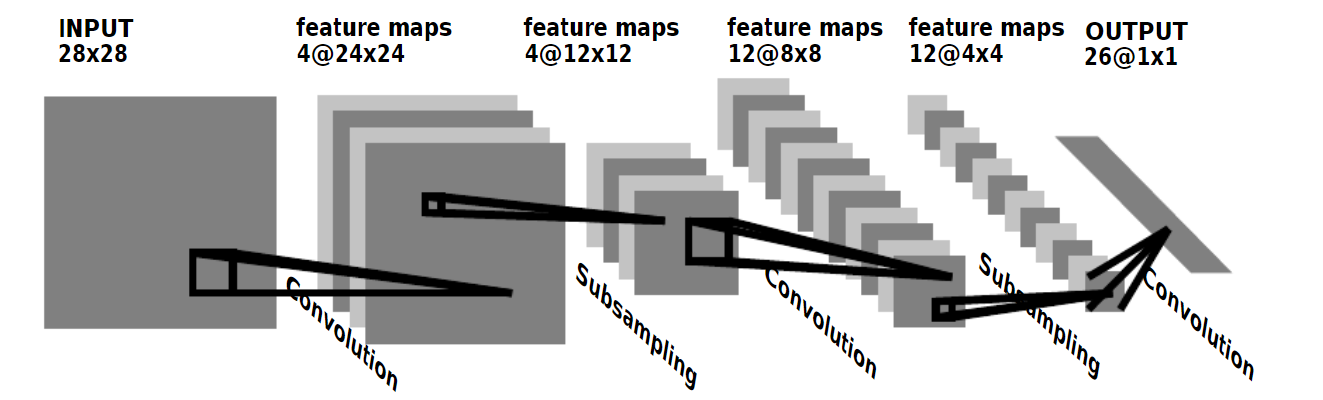
\includegraphics[width=\textwidth]{images/CNN.png}
  \caption{Exemple de représentation schématique d'un réseau de neurones convolutif \cite{articleCNN}}
  \label{fig:CNN}
\end{figure}


Les CNN sont formés de 3 types de couches principales :\\

\begin{itemize}
\item les couches de convolution : ce sont les bases d'un CNN, elles permettent d'extraire les caractéristiques d'une image et font l'effet de filtre sur l'image en entrée. Chaque neurone d'une couche de convolution dispose d'un noyau appliqué sur toute l'image et dont les valeurs seront optimisées par l'entraînement. Les hyperparamètres associés à ces couches sont : la profondeur de la couche (c'est à dire le nombre de noyaux de convolution qui produiront chacun une image filtrée), la taille des noyaux, le stride qui correspond au nombre de pixels entre chaque déplacement du noyau et le padding qui rajoute des pixels de valeurs nulles afin de conserver les dimensions des images obtenues en sortie.\\

\item les couches de pooling : elles consistent à réduire la taille spatiale des images intermédiaires afin de limiter les calculs du modèle tout en conservant l'information. Pour cela, l'image d'entrée est découpée en série de rectangles de même taille auxquels on applique une fonction sur l'ensemble de leurs pixels pour n'en obtenir qu'un seul par rectangle dans l'image finale. Les techniques de pooling les plus souvent utilisées sont le max-pooling et le average-pooling.\\

\item les couches complètement connectées (fully-connected) : ce sont les couches finales d'un CNN. Elles prennent en entrée les réponses aux filtres aplatis en un seul et même vecteur. Ces couches suivent le même principe que celui expliqué en \ref{subsubsec:ANN} et permettent de décider de la classe prédite par le modèle. Le nombre de neurones de la dernière couche sera donc égal au nombre de classes possible du dataset d'entrée. Pour obtenir une probabilité, la fonction d'activation softmax est souvent privilégiée.\\
\end{itemize}



\subsection{Exemple du ResNet}
\label{subsec:renet}
L'arrivée des CNN dans la résolution des problèmes de classification a été une avancée majeure dans le domaine qui a conduit à d'excellents résultats pour des réseaux de convolution très profonds. Cependant, cela a soulevé la question de l'efficacité de constamment augmenter le nombre de couches de ces réseaux afin de résoudre des problèmes de classification toujours plus complexes en nombre de classes et en proximité visuelle. En effet, pour des réseaux profonds pouvant converger, à mesure que leur profondeur augmente, leur précision est impactée négativement et cela n'est ni expliqué par des problèmes de surapprentissage, ni même par le phénomène d'explosion ou de disparition du gradient \cite{he2015deep}. En effet, ceux-ci sont résolus par l'initialisation normalisée \cite{LeCun1998} et les couches intermédiaires de normalisation \cite{ioffe2015batch}. \\

Un moyen de mieux optimiser le problème, et ainsi résoudre les pertes de précision avec la profondeur, a été l'introduction des réseaux neuronaux résiduels dont le principe est d'entraîner la sortie de la couche précédente mais également un résidu d'une couche précédente \cite{he2015deep}. Les architectures utilisant cette méthode sont aussi appelées ResNet. Elles utilisent des blocs avec des connexions raccourcies sautant une ou plusieurs couches (figure \ref{fig:residual_bloc}).\\


\begin{figure}[ht]
    \centering
    
    \begin{tikzpicture}[->,>=latex,node distance=4cm]
    
    
        \tikzstyle{layer} = [draw, rectangle, minimum size=1cm, minimum width=3cm, text centered];
        \tikzstyle{weight} = [draw, >=stealth, shorten >=0.5pt];
        
        \node[layer] (l2) {Couche $i-2$};
        \node[layer] (l1) [right of=l2] {Couche $i-1$};
        \node[layer] (l) [right of=l1] {Couche $i$};
        \coordinate[left of=l2] (c1);
        \coordinate[right of=l] (c2);
        \path[every node/.style={font=\sffamily\small}]
            (c1) edge node [below] {} (l2)
            (l2) edge node [below] {} (l1)
            (l1) edge node [below,label=:{$Z^i$}] {} (l)
            (l) edge node [below, label=:{$a^i$}] {}(c2)
            (l2.east) edge[bend left=70] node [below,label=below right :{$W^{i-2,i}a^{i-2}$}] {} (l.north west);
        
    \end{tikzpicture}
    
    \caption{Bloc d'un réseau neuronal résiduel}
    \label{fig:residual_bloc}
\end{figure}

De manière plus formelle, pour une couche $i$ quelconque qui reçoit un résidu, on a donc
$$
a^i = g(W^{i-1,i}a^{i-1}+b^i+W^{i-2,i}a^{i-2}) = g(Z^i+W^{i-2,i}a^{i-2})
$$
avec $a^i$ les sorties des neurones de la couche $i$, $g$ la fonction d'activation pour la couche $i$, $b^i$ le vecteur de biais associé à la couche et $W^{i-1,i}$ la matrice de poids entre les couches $i-1$ et $i$.\\

L'architecture originale de ResNet est le ResNet-34, qui comprend 34 couches (figure \ref{fig:ResNet_34}). Il a été conçu avec ses frères de 50, 101 et 151 couches pour classifier les images du célèbre jeu de données ImageNet. C'est l'architecture qui remportera le concours 2015 organisé par l'organisation derrière ImageNet. \\

Au cours de notre projet nous avons utilisé l'implémentation officielle sur pytorch de l'architecture de 50 couches (ResNet-50) qui dispose d'une avant-dernière couche d'average pooling (sorties de taille 2048) et d'une dernière couche complètement connectée vers les 1000 sorties (correspondant aux 1000 classes).

\begin{figure}[ht]
  \centering
  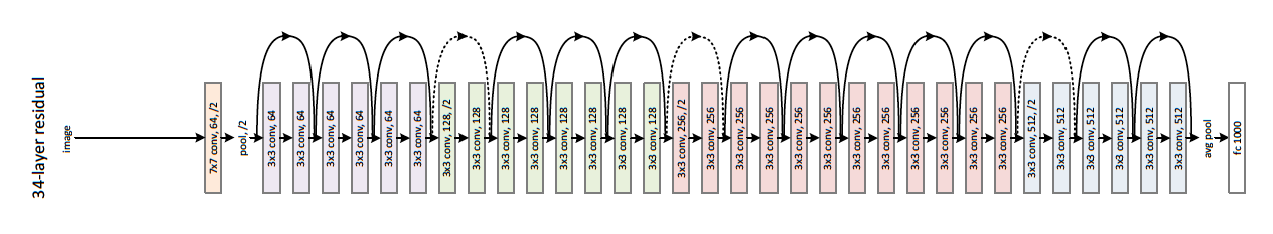
\includegraphics[width=\textwidth]{images/resNet3.png}
  \caption{Exemple d'architecture pour ImageNet : ResNet comprenant 34 couches \cite{he2015deep}}
  \label{fig:ResNet_34}
\end{figure}

\section{L'impact de la régularisation sur l'apprentissage dépend des classes}

Pour réduire le problème de surapprentissage et contrôler la complexité des modèles utilisés en machine learning ou en statistiques, la régularisation est fréquemment utilisée. Elle consiste à restreindre l’espace de recherche des solutions pendant la phase d’apprentissage pour imposer aux paramètres de rester petits. En deep learning, la régularisation peut être effectuée de plusieurs manières : soit explicitement en pénalisant les poids (traduit par l'utilisation d'un weight decay) ou soit implicitement en utilisant d’autres techniques comme l’augmentation de données.\\ 

En deep learning, les problèmes de classification consistent à considérer plusieurs classes auxquelles en fonction d’une entrée quelconque (image, texte) le classifieur attribuera autant de nombres en sortie qu’il y a de classes, chacun compris dans un intervalle, typiquement $[0, 1]$. Cependant, ces problèmes demandent souvent plusieurs centaines ou milliers de classes ce qui augmente considérablement la complexité des modèles.\\

Balestriero et al. (2022) \cite{NEURIPS2022_f73c0453} ont démontré récemment qu'en utilisant une régularisation comme le weight decay, un biais significatif est ajouté dans le modèle entraîné. Malgré l'amélioration globale de la précision du modèle, il y a alors une inégalité entre la précision relative à chacune des classes, c'est à dire que certaines classes voient leur précision diminuer arbitrairement. Le weight decay choisi fait alors le compromis entre toutes les classes mais n'est optimal pour aucune d'entre elles (illustration fidure \ref{fig:class_inequalities}).
\begin{figure}[ht]
  \centering
  \includesvg[width=12cm]{images/class_inequalities.svg}
  \caption{Ensemble de 3 classes prisent arbitrairement pour témoigner de la performance de la validation croisée qui est plutôt bonne sur la majorité des classes mais relativement mauvaise sur les autres quand la complexité du modèle est calibrée par une régularisation (ici le weight decay) }
  \label{fig:class_inequalities}
\end{figure}


\chapter{La dernière représentation interne du modèle d'apprentissage profond, décisive dans la classification }
\section{Notations}
\label{sec:Nota1}
Dans la suite de ce rapport nous aurons recours à des conventions de notations spécifiques, introduisons : \\

\begin{itemize}
    \item $K$ le nombre de classes possibles identifiables\\
    \item $n$ le nombre de couches du  réseau de neurones\\
    \item $w^{[i]}_{o_1,o_2} \in \mathbb{R}$ la valeur du poids liant le $o_2^{eme}$ neurone de la couche $i$ avec le $o_1^{eme}$ neurone de la couche $i-1$ du réseau\\
    \item $z_o^{[i]}$ la valeur que reçoit en entrée le $o^{eme}$ neurone de la couche $i$ : la somme des sorties pondérées de la couche $i-1$, on notera $z^{[0]}_o$ les entrées du réseau de neurones\\
    \item $a_o^{[i]}$ la valeur de sortie d'une $o^{eme}$ neurone de la couche $i$ \\
    \item $\hat{y}_c$ la prédiction associée au neurone $c$ de la dernière couche, avec $c \in [0, K]$, l'indice d'un neurone de la dernière couche (équivalent à l'indice de la classe) \\
    
\end{itemize}

\section{Importance de la dernière couche}
\label{sec:lastlayer}

Dans les réseaux de neurones convolutifs, les couches complètement connectées (section \ref{subsec:CNN}) viennent après les couches de convolutions, de pooling et de correction. L'ensemble des couches complètement connectées prend donc en entrée les représentations apprises par les précédentes couches sous forme d'un unique vecteur en 1D. Ce sont ces couches où la décision finale est prise quant à la prédiction du modèle. Pour un problème de classification comme le nôtre, c'est à l’issue de cet ensemble complètement connectées que la classe à laquelle appartient l'image est prédite.\\

Au cours de notre étude, le modèle utilisé est le ResNet-50 (section \ref{subsec:renet}) composé de couches de convolution et de pooling suivies d'une unique dernière couche complètement connectée avec une fonction d'activation softmax permettant ainsi d'estimer la probabilité de la classe de l'image passée en entrée du modèle. Par conséquent, c'est cette couche qui est déterminante dans le résultat final et dans la bonne estimation du modèle. Les couches précédentes permettent d'extraire les caractéristiques de l'image et de les représenter de manière résumée en un seul vecteur 1D.\\

L'implémentation officielle du ResNet-50 fourni par Pytorch dispose d'une dernière couche de 1000 neurones correspondant au nombre de classes et d'un vecteur d'entrée de taille 2048 pour cette couche finale.

\section{Limitations}
\label{sec:limitations}
Dans le cadre de notre étude, pour pouvoir entraîner notre modèle profond, il est nécessaire de disposer de puissants GPU pour accélérer au mieux les calculs. Cependant, dans le cas contraire, il est déraisonnable d'un point de vue temporel d'essayer cet entraînement dénué de puissants GPU.\\

Dans le cadre de notre étude c'est principalement la dernière couche qui nous intéresse (section \ref{sec:lastlayer}) car c'est la prise de décision qu'on souhaite étudier et optimiser. Pour ce faire, deux options sont alors possibles pour utiliser le modèle pré-entraîné pour toutes les couches mis à part les dernières, complètement connectées. La première consiste à empêcher l'apprentissage sur ces couches en bloquant la rétropropagation du gradient.\\

Cependant, la limite de cette méthode est le coût en calcul de l'évaluation du modèle pendant l'entraînement qui n'est pas négligeable au vu du nombre important de couches du réseau. La deuxième option est celle qu'on a privilégiée, elle consiste à évaluer la sortie de la couche précédant la première couche complètement connectées du modèle pour chacune des images du dataset d'entraînement (correspondant à la sortie de l'avant dernière couche du ResNet-50). À partir de ces sorties, on entraîne un modèle de régression logistique séparément afin de simuler l'effet des couches complètement connectées en évitant les calculs redondants des premières couches pendant l'entraînement.

\section{Évaluation du modèle}

Pour obtenir le dataset composé des sorties de la couche précédant les couches complètement connectées, il est nécessaire d'évaluer notre modèle pour chaque image de l'ensemble d'ImageNet en calculant la propagation du ResNet pré-entraîné.

\subsection{ImageNet}
\label{subsec:ImageNet}
ImageNet est un projet créé par des chercheurs de l'Université de Stanford et de l'Université de Princeton en 2009 dont l'objectif est de constituer une base de données de plusieurs millions d'images différentes afin de permettre aux chercheurs du monde entier d'y accéder librement pour faire avancer la recherche sur les modèles de deep learning de vision. Pour atteindre cet objectif, les chercheurs ont collecté plus de 14 millions d'images à partir de diverses sources, telles que des moteurs de recherche et des sites Web d'images libres de droits.\\

Chaque image a été annotée manuellement avec l'une des 21 841 catégories issues de la hiérarchie WordNet, une base de données lexicale qui regroupe les mots en groupes de synonymes cognitifs (synsets) exprimant des concepts distincts. Ces synsets sont interconnectés sémantiquement par un réseau de relations conceptuelles comme la relation d'hyperonymie/hyponymie qui relie les concepts généraux aux plus spécifiques (ex : meuble -> lit -> lit superposé).\\

Le projet d'ImageNet a aussi donné lieu à la compétition annuelle ILSVRC (2010-2017) qui a permis de jouer un rôle essentiel dans le développement de modèles de réseau de neurones convolutifs (CNN) tels que AlexNet, VGG, et ResNet qu'on a utilisé dans le cadre de notre expérience avec sa version de 50 couches.
\subsection{Propagation}

Pour les couches complètement connectée d'un réseau de neurones (section \ref{subsubsec:ANN}) appelées aussi couches denses, pour obtenir la prédiction du modèle étant donné une entrée $z^[0]$, on effectue la propagation en avant caractérisée par l'équation suivante utilisée à chaque neurone $o$ de la couche $i$ du modèle : 

$$
    z_{o}^{[i]} = \sum_{p} w^{[i]}_{p,o}a_{p}^{[i-1]}
$$
En sortie du modèle, l'a fonction d'activation utilisée est la fonction softmax pour obtenir une probabilitée, caractérisée par l'expression suivante :
$$
    \hat{y}_c = \frac{\exp{z_{c}^{[n]}}}{\sum_{o}\exp{z_{o}^{[n]}}}
$$
Le vecteur $\hat{y}$ ainsi obtenu correspond à l'ensemble des prédictions de chacune des classes sous forme de probabilité lorsqu'on est dans un problème de classification.

\subsection{Sauvegarde des poids}
\label{subsec:save_weights}
Dans un premier temps, étant donné que l'entraînement et la simple évaluation de millions d'images dans un réseau de neurones profond comme un ResNet-50 est très coûteuse, le plus efficace est d'évaluer les sorties de taille $n$ (dans notre cas, $n=2048$) obtenues à l'avant-dernière couche du réseau pour chacune des images de l'ensemble de données d'entraînement (dans notre cas, ImageNet), et de sauvegarder ces résultats dans un dataset qui servira par la suite à entraîner notre modèle de régression logistique. (cf. section \ref{sec:limitations})\\

En effet, étant donné que l'objectif est d'étudier l'évolution de la fonction de coût pour chacune des classes au cours de l'apprentissage, il est nécessaire de sauvegarder les modèles à différentes époques de l'apprentissage et surtout pour différents hyperparamètres de régularisation. 

\subsection{Algorithme utilisé}

Pour implémenter la sauvegarde des sorties de l'avant-dernière couche de notre modèle, nous avons utilisé la librairie "pytorch", voici un exemple simplifié, extrait du code source utilisé : 

\begin{minted}[fontsize=\footnotesize]{python}
# Instanciation du modèle ResNet-50 avec les poids par défaut
model = resnet50(weights=ResNet50_Weights.DEFAULT)

# Définition du dictionnaire de stockage des activations 
activation = {}
def getActivation(name):
  '''
  Fonction pour le forward hook afin de récupérer 
  les sorties de l'avant dernière couche.
  '''
  def hook(model, input, output):
    activation[name] = output.detach()
  return hook

h = model.avgpool.register_forward_hook(getActivation('avgpool'))
dataloader = DataLoader(
    dataset, 
    batch_size=batch_size, 
    num_workers=num_workers, 
    pin_memory=pin_memory
)
# Début de la propagation en avant sans calculer les gradients
model.eval()
with torch.no_grad():
    # Itérations sur les batchs fournis par le dataloader
    for images, labels in tqdm(dataloader, desc="Evaluation"):
        
        outputs = model(images) # Calcul des prédictions faites par le modèle

        # Récupération des activations de l'avant-dernière couche (average pooling)
        avgpool_list = torch.cat([avgpool_list, activation['avgpool'].squeeze()],dim=0) 
         
torch.save(avgpool_list, f'{saving_folder}.pt') 
\end{minted} 

\chapter{Apprentissage d'un modèle de régression logistique multinomiale}
\section{Notations}
Nous reprendrons les notations introduites en section \ref{sec:Nota1}.

\section{Un modèle de régression logistique multinomiale}
\label{sec:model_reg_log_multi}
Dans le domaine de l'apprentissage automatique (Machine Learning), on distingue généralement deux grands types d'algorithmes : l'apprentissage supervisé et l'apprentissage non supervisé. L'objectif est de déterminer une fonction $f$ qui modélise au mieux la relation entre les données d'entrée et les données de sortie, de sorte que :

$$sortie = f(entrée)$$

Dans le cas de l'apprentissage supervisé, les données d'entraînement comprennent les étiquettes (labels) correspondant aux sorties désirées. Les problèmes d'apprentissage supervisé peuvent être divisés en deux catégories principales : la régression et la classification.\\

La régression est utilisée lorsque la variable cible est continue, tandis que la classification est employée lorsque la variable cible est discrète, c'est-à-dire qu'elle prend un nombre fini de valeurs distinctes (modalités). Dans le cas présent, les sorties étant discrètes, un modèle de classification est approprié.\\

La régression logistique est un modèle de classification souvent utilisé pour modéliser la probabilité d'appartenance à chaque classe. Elle est particulièrement adaptée aux problèmes binaires (deux classes), mais peut être généralisée à des problèmes multiclasses (plusieurs modalités) sous la forme de la régression logistique multinomiale que nous utiliserons pour simuler la dernière couche du ResNet-50.\\

Soit $\mathbf{x} = (x_1, x_2, \ldots, x_N)$ le vecteur d'entrée de taille N. La couche linéaire applique une transformation affine à ce vecteur d'entrée pour produire un vecteur de scores non normalisés $\mathbf{z} = (z_1, z_2, \ldots, z_K)$ de taille K, correspondant aux K classes. Cette transformation est réalisée à l'aide d'une matrice de poids $\mathbf{W}$ de taille $N \times K$ et d'un vecteur de biais $\mathbf{b}$ de taille $K$, selon l'équation suivante :

$$\mathbf{z} = \mathbf{W}^\top\mathbf{x} + \mathbf{b}$$

La fonction d'activation softmax est ensuite appliquée au vecteur de scores non normalisés $\mathbf{z}$ pour obtenir un vecteur de probabilités $\mathbf{\hat{y}}$ de taille $K$, où chaque élément $\hat{y_i}$ représente la probabilité estimée que l'entrée $\mathbf{x}$ appartienne à la classe $i$. La fonction softmax est définie comme suit :

$$\hat{y_i} = \frac{e^{z_i}}{\sum_{j=1}^{K} e^{z_j}}$$

Lors de l'entraînement du modèle, la fonction de coût de l'entropie croisée est minimisée pour ajuster les paramètres $\mathbf{W}$ et $\mathbf{b}$. L'entropie croisée $\mathcal{L}$ entre les probabilités prédites $\mathbf{\hat{y}}$ et les étiquettes réelles $\mathbf{y}$ (sous forme de vecteur one-hot de taille K - vecteurs composés de une seule valeur égale à 1, les autres nulles) est définie comme :

$$
\mathcal{L}(\mathbf{y}, \mathbf{\hat{y}}) = - \sum_{j = 1}^{K} y_{j} \log \hat{y}_{j}
$$

On cherchera ainsi à minimiser cette fonction par la suite.

\section{Entraînement}

À partir des sorties de l'avant-dernière couche du modèle initial (ResNet-50), on constitue un nouvel ensemble de données (voir section \ref{subsec:save_weights}) composé d'autant de vecteurs qu'il y avait d'images initialement. Par conséquent, on défini un modèle de régression logistique multinomial composé d'une seule couche de sorties complètement connectée (explications section \ref{sec:limitations}) qu'on entraîne avec le nouveau dataset des vecteurs de l'avant-dernière couche obtenu. L'ajustement des valeurs des poids permet ensuite de minimiser la fonction de perte et ainsi obtenir un taux de bonne classification optimal.\\

L'entraînement d'un tel modèle consiste à trouver la valeur des poids permettant d'avoir une fonction de coûts minimale. Dans notre cas, on utilisera l'entropie croisée $\mathcal{L}$ définit pour le vecteur $\mathbf{y}$ correspondant au label de taille $K$ associée au vecteur d'entrée $\mathbf{x}$ et $\mathbf{\hat{y}}$ la prédiction obtenue par le modèle (section \ref{sec:model_reg_log_multi}):
$$
\mathcal{L}(\mathbf{y}, \mathbf{\hat{y}}) = - \sum_{j = 1}^{K} y_{j} \log \hat{y}_{j}
$$
avec $y_{j}$ et $\hat{y}_{j}$ les valeurs d'indice $j$ des vecteurs $\mathbf{y}$ et $\mathbf{\hat{y}}$ respectivement.\\

Ensuite, afin de limiter le surapprentissage mais également dans le cadre de notre projet, nous rajoutons un weight decay en utilisant la régularisation L2 (ie. section \ref{subsec:regularisation}) afin d'obtenir la fonction de coût $L2$ que l'algorithme minimisera : 

$$
L2(\mathbf{y}, \mathbf{\hat{y}}) = \mathcal{L}(\mathbf{y}, \mathbf{\hat{y}}) + \frac{\lambda }{2}\lVert \mathbf{w}\rVert ^2
$$

avec $\lambda \geq 0$ l'hyperparamètre de régularisation, et $\mathbf{w}$ le vecteur de poids de l'unique couche du réseau.\\

L'intérêt de cette méthode est d'étudier l'impact de la technique de régularisation utilisant un weight decay sur l'apprentissage de notre modèle pour différentes classes et pour différentes valeurs de cet hyperparamètre.\\

Au cours de l'entraînement, il est également intéressant de recueillir les valeurs des erreurs et de la fonction optimisée à chaque époque afin de détecter de potentiels phénomènes de surapprentissage ou de sous-apprentissage.

\subsection{Backpropagation et descente de gradient}
\label{subsec:backprop}
\subsubsection{Généralisation}
Le processus d'entraînement et d'ajustement des poids d'un réseau de neurones à propagation avant (légèrement différent pour un réseau neuronal résiduel) est caractérisé d'abord par l'algorithme de backpropagation qui calcule les gradients de la fonction de coût en utilisant la règle de dérivation en chaîne. Pour cela, l'algorithme propage l'erreur en arrière et calcule le gradient de la fonction de coût. Les explications mathématiques du processus sont décrites ci-dessous.\\\\
Soit $\mathcal{L}$ la fonction de coût.
On a pour la dernière couche :
$$
    \frac{\partial{\mathcal{L}}}{\partial{z_{o}^{[n]}}} = \sum_c \frac{\partial{\mathcal{L}}}{\partial\hat{y}_c}\frac{\partial\hat{y}_c}{\partial{z_{o}^{[n]}}} = \hat{y}_o - y_o
$$
\begin{tabbing}
\hspace{2cm}
car 
\end{tabbing}
\begin{align*}
&\frac{\partial{\mathcal{L}}}{\partial\hat{y}_c} = - \frac{y_c}{\hat{y_c}}
&&\frac{\partial\hat{y}_c}{\partial{z_{o}^{[n]}}} = \left\{
\begin{array}{cc}
     \frac{e^{z_{c}^{[n]}}}{\sum_{o}^{}e^{z_{o}^{[n]}}} - \frac{e^{z_{c}^{[n]}}e^{z_{c}^{[n]}}}{(\sum_{o}^{}e^{z_{o}^{[n]}})^2} =  \hat{y}_c(1- \hat{y}_c) & \mbox{si } c = o  \\\\
     0 - \frac{e^{z_{c}^{[n]}}e^{z_{c}^{[n]}}}{(\sum_{o}^{}e^{z_{o}^{[n]}})^2} = - \hat{y}_c\hat{y}_o & \mbox{si } c \neq o
\end{array}
\right.
\end{align*}
\begin{tabbing}
\hspace{2cm}
donc,

\end{tabbing}
$$
\frac{\partial{\mathcal{L}}}{\partial w^{[n]}_{p,o}} = \frac{\partial{\mathcal{L}}}{\partial{z_{o}^{[n]}}}\frac{\partial{z_{o}^{[n]}}}{\partial w^{[n]}_{p,o}} = (\hat{y}_o - y_o)a_p^{[n-1]}
$$

On a pour la $i^{eme}$ couche :
$$
\frac{\partial{\mathcal{L}}}{\partial w^{[i]}_{q,p}} = \sum_o \frac{\partial{\mathcal{L}}}{\partial z_{o}^{[i+1]}} \frac{\partial{z_{o}^{[i+1]}}}{\partial{a_{p}^{[i]}}} \frac{\partial{a_{p}^{[i]}}}{\partial{z_{p}^{[i]}}} \frac{\partial{z_{p}^{[i]}}}{\partial w^{[i]}_{q,p}} = \sum_o (\hat{y_o} - y_o) w^{[i+1]}_{p,o}a^{[i]}_{p}(1-a_{p}^{[i]})a_{q}^{[i-1]}
$$

A l'issu de l'algorithme de backpropagation, après avoir calculé le gradient, on utilise l'algorithme d'optimisation de descente de gradient pour trouver les nouveaux poids qui minimiseront la fonction de coût (en réalité on utilise la descente de gradient stochastique par minibatch (SGD) qui, au lieu de parcourir tous les échantillons de l'ensemble d'apprentissage pour effectuer une seule mise à jour des paramètres, utilise uniquement un sous-ensemble ou batch afin de réduire considérablement le temps de calcul tout en conservant des performances acceptables). La formule qui caractérise la descente de gradient est la suivante,

$$
    w^{[i]}_{o,p} = w^{[i]}_{o,p} - \alpha \frac{\partial \mathcal{L}}{\partial w^{[i]}_{o,p}} 
$$

avec $\alpha$ le pas de gradient (learning rate) tel que $\alpha \geq 0$.

\subsubsection{Optimisations particulières}

La première optimisation qu'on utilise communément est l'usage d'un step scheduler pour le learning rate qui va permettre de réduire la valeur du learning rate d'un facteur à chaque intervalle d'époques de l'apprentissage afin d'améliorer la stabilité et la précision du modèle en le faisant converger plus en douceur. Grâce à cette méthode, on permet au modèle d'apprendre suffisamment rapidement pendant les premières époques de l'apprentissage puis en réduisant l'amplitude des mises à jour à mesure que le modèle converge, cela permet d'améliorer encore plus précisément les poids au lieu d'osciller autour de l'optimum.\\

Une autre optimisation intéressante pour l'apprentissage est l'usage de la descente de gradient avec un "momentum". L'objectif de cette technique est d'accélérer le processus d'apprentissage pour atteindre le point de convergence. En effet, le problème avec l'algorithme de la descente de gradient est que sur les pentes douces, le gradient devient très faible et les mises à jour deviennent lentes. L'utilisation d'un momentum consiste à utiliser la mise à jour précédente d'un poids multipliée par un nouvel hyperparamètre auquel on ajoute le terme calculé avec la backpropagation. Ce comportement ce traduit ainsi par les équations :


$$
(b^{[i]}_{o,p})_t = \mu \cdot (b^{[i]}_{o,p})_{t-1} + \frac{\partial \mathcal{L}}{\partial w^{[i]}_{o,p}}
$$ 
$$
w^{[i]}_{o,p} = w^{[i]}_{o,p} - \alpha (b^{[i]}_{o,p})_t
$$
avec $\mu$ le nouvel hyperparamètre associé au momentum et $(b^{[i]}_{o,p})_t$ le terme modifié de direction pour le poids $w^{[i]}_{o,p}$ à une période $t\in \mathbb{N}$ donnée de l'apprentissage.



\subsection{Régularisation : weight decay}
\label{subsec:regularisation}
Le weight decay est une méthode de régularisation qui est utilisée pour pénaliser la fonction de coût pour réduire l’amplitude des poids et les empêcher de devenir trop importants. Cela permet de limiter le surapprentissage. En effet, des poids élevés provoquent une variance élevée en sortie. Pour cela, la fonction de coût est pénalisée. Il se décline de deux façons :\\

\begin{enumerate}
     
\item L1 Regularisation : \\

Combat le sur-apprentissage en réduisant les poids de certaines caractéristiques à 0. Cela revient à sélectionner certaines caractéristiques et en supprimer d'autres.
$$L1\; Regularisation = (fonction\; de\; perte) + \lambda\sum_{i=1}^{n}\sum_{p=1}^{m_i}\sum_{o=1}^{m_{i-1}} |w^{[i]}_{o,p}|$$
avec $n$ le nombre de couche, $m_i$ le nombre de neurone de la couche $i$ et $\lambda \geq 0$\\

\item L2 Regularisation :\\

Combat le sur-apprentissage en réduisant les poids de certains caractéristiques mais les poids restent supérieur à 0. Ainsi les caractéristiques moins importantes auront toujours une une petite influence sur la prédiction.
$$L2\; Regularisation = (fonction\; de\; perte) + \lambda\sum_{i=1}^{n} \lVert \mathbf{w}^{[i]}\rVert^2$$
avec $\lambda \geq 0$ et $\mathbf{w}^{[i]}$ le vecteur de poids de la couche $i$
du modèle.\\

\item Comparaison des 2 méthodes :\\

\begin{itemize}
    \item La L1 Regularisation renvoie une solution clairsemée alors que la L2 Regularisation une solution dense.
    \item La L1 Regularisation offre une solution plus robuste alors que L2 Regularisation offre une solution moins coûteuse en calcul.\\
\end{itemize}

Pour notre problème nous opterons pour la régularisation L2 implémentée nativement de cette manière avec l'optimiseur SGD de pytorch.

\end{enumerate}

\section{Algorithme pour l'entraînement du modèle}

Pour implémenter l'apprentissage et l'instanciation du modèle de régression logistique, toujours avec pytorch, nous avons définit une classe personnalisée, voici un exemple simplifié, extrait et adapté du code source réellement utilisé :

\begin{minted}[fontsize=\footnotesize]{python}
# Initialisation d'une classe personnalisée pour avoir un dataset optimisé sur les 
# sorties de l'avant dernière couche du ResNet-50 sur ImageNet (voir code source)
dataset = PenultimateOutputsDataset(outputs_folder)
train_loader = DataLoader(dataset, batch_size=batch_size, pin_memory=True)

torch.manual_seed(0) # Reproductibilité de l'expérience dans l'initialisation aléatoire des poids
 
class LogisticRegression(nn.Module): 
    '''
    Implémentation du modèle de régression logistique avec torch
    '''
    def __init__(self, input_size, num_classes): 
        super(LogisticRegression, self).__init__()
        # Définition de la couche linéaire
        self.linear = nn.Linear(input_size, num_classes) 
  
    def forward(self, x):
        # Définition de la propagation en avant
        out = self.linear(x) 
        return out

# Itérations sur les différents weights decay
for weight_decay_parameter in weight_decay_parameters :
    
    # Définition du modèle
    model = LogisticRegression(input_size=input_size, num_classes=num_classes) 

    # Définition de la fonction de loss et de l'optimiseur
    loss_function = nn.CrossEntropyLoss() # softmax intégrée à la fonction
    optimizer = torch.optim.SGD(
        model.parameters(), 
        lr=learning_rate, 
        momentum=momentum, 
        weight_decay=weight_decay_parameter
    )

    # Définition du scheduler pour faire varier le learning rate
    scheduler = torch.optim.lr_scheduler.StepLR(
        optimizer, 
        step_size=lr_decay_step, 
        gamma=decay_rate
    )
    
    # Initialisation des différentes variables pour stocker les éléments intéressants
    accuracy_history = []
    L2_regularisation_history = torch.tensor([])
    mean_loss_class = torch.tensor([])
    weights_epoch = torch.tensor([])

    # Obtention du nombre d'images par classe
    nb_image_class = torch.bincount(dataset.labels).to(DEVICE)
    
    for epoch in range(num_epochs): 
            
        # Initialisation du nombre de prédictions correctes
        correct_predictions = 0
    
        # Initialisation du vecteur de la somme des valeurs de la fonction de coût pour chaque classe
        class_loss = torch.zeros(1000)
        
        for inputs, labels in train_loader:
        
            # Forward pass 
            outputs = model(inputs) 
            loss = loss_function(outputs, labels)
            L2_regularisation = loss + weight_decay_parameter * \ 
            sum(t.pow(2).sum() for t in model.state_dict().values()) / 2
    
            # Calcul de la fonction de coût pour chaque image et ajout dans class_loss
            input_loss = nn.functional.cross_entropy(outputs,labels,reduction='none') + \
            weight_decay_parameter * sum(t.pow(2).sum() for t in model.state_dict().values()) / 2
            # On obtient ainsi la valeur de la fonction de coût pour chaque classe
            class_loss.index_add_(0,labels,input_loss)
            
            # Ajout des prédictions correctes au total
            _, predicted = torch.max(outputs, 1)
            correct_predictions += (predicted == labels).sum().item()
    
            # Backpropagation et optimisation 
            optimizer.zero_grad() 
            loss.backward() 
            optimizer.step()
        
        # Modification du lerning rate
        scheduler.step()
    
        # Sauvegarde du modèle intermédiaire 
        # (models_path normalement défini et modifié pour chaque weight decay) 
        torch.save(model.state_dict(), f'{models_path}/epoch-{epoch}.pt')
    
        # Calcul du taux de bonne classification
        accuracy = 100 * correct_predictions / len(dataset)
    
        # Sauvegarde des différentes mesures
        accuracy_history.append(accuracy)
        L2_regularisation_history = torch.cat(
            (L2_regularisation_history, L2_regularisation.unsqueeze(0)), 
            dim=0
        )
        mean_loss_class = torch.cat(
            (mean_loss_class,(class_loss/nb_image_class).detach().unsqueeze(0)), 
            dim=0
        )
        weights_epoch = torch.cat(
            (weights_epoch, sum(t.abs().sum() for t in model.state_dict().values()).unsqueeze(0)), 
            dim=0
        )
            
    # Sauvegarde de toutes les données importantes liées à l'entraînement du modèle
    # (data_path normalement défini et modifié pour chaque weight decay)
    torch.save(accuracy_history, f'{data_path}/accuracy.pt')
    torch.save(loss_history, f'{data_path}/loss.pt')
    torch.save(L2_regularisation_history, f'{data_path}/L2_regularisation.pt')
    torch.save(mean_loss_class, f'{data_path}/mean_loss_class.pt')
    torch.save(weights_epoch, f'{data_path}/weights.pt')

\end{minted}

\section{Interprétation des résultats}

Pour visualiser les différences sur les prédictions selon le choix du paramètre du weigh decay ($\lambda$), on trace la fonction de coût et le taux de bonne classification en fonction des époques du modèle.
\subsection{Définition}
\subsubsection{Taux de bonne classification}
Le taux de bonne classification est un facteur déterminant dans le choix du modèle. En effet, plus le taux de bonne classification est grande : meilleur est notre modèle. Pour chaque modèle, elle se calcule de cette facon :
$$
    Taux\; de\; bonne\; classification = \frac{1}{n_d}\sum_{i=1}^{n_d} \mathbb{1}_{y_i = \hat{y}_i}
$$
avec $n_d \in \mathbb N$ le nombre d'images.\\


\subsubsection{Fonction de coût}
La fonction de coût est aussi un facteur déterminant dans le choix du modèle. De plus, elle est utilisée dans la descente de gradient (Voir section \ref{subsec:backprop}) et dans l'apprentissage de notre modèle. Pour chaque modèle, elle se calcule de cette façon :
$$
\mathcal{L}(\mathbf{y}, \mathbf{\hat{y}}) = - \sum_{j = 1}^{K} y_{j} \log \hat{y}_{j} 
$$
avec $y_{j}$ et $\hat{y}_{j}$ les valeurs d'indice $j$ des vecteurs $\mathbf{y}$ et $\mathbf{\hat{y}}$ respectivement.

\subsection{Analyse}

\begin{figure}[H]
    \centering
  \subfigure[Taux de bonne classification en fonction des époques]{\includesvg[width=\linewidth, height=0.3\textheight]{images/accuracy_epoch_wd_train.svg}}\hfill
  \subfigure[Fonction de coût en fonction des époques]{\includesvg[width=\linewidth, height=0.3\textheight]{images/loss_function_epoch_wd_train.svg}\label{fig:result_train_epoque_cout}}\hfill
  \subfigure[L2 Regularisation en fonction des époques]{\includesvg[width=\linewidth, height=0.3\textheight]{images/L2_Regularization_epoch_wd_train.svg}\label{fig:result_train_epoque_L2}}\hfill
  \caption{Évolution des résultats pour l'ensemble d'entraînement sur les modèles obtenus à l'issu de chaque époque de l'entraînement}
  \label{fig:result_train_epoque}
\end{figure}

En premier lieu, la figure \ref{fig:result_train_epoque_L2} témoigne du bon déroulement de l'apprentissage. En effet, la régularisation L2, tracée en ordonnée, est la fonction minimisée pendant le processus d'entraînement qui va décroître au cours de l'apprentissage. Les paliers témoignent de la variation brutale du pas de gradient qui permet à l'algorithme de sortir d'un potentiel état oscillant autour de l'optimum pour ainsi diminuer directement la valeur de l'erreur. Les valeurs $\lambda$ de weight decay les plus élevés témoignent d'une importante pénalisation qu'on retrouve dans nos expériences avec l'écart entre les valeurs de la fonction de régularisation. Cette pénalisation se traduit par des performances réduites au cours de l'apprentissage pour éviter au modèle d'être ajusté spécifiquement pour l'ensemble d'entraînement. En comparant la figure \ref{fig:result_train_epoque_L2} à la figure \ref{fig:result_train_epoque_cout}, on en déduit la présence du terme de régularisation qui augmente les valeurs à la dernière époque. Cependant, contrairement à la figure \ref{fig:result_train_epoque_L2} les courbes de la figure \ref{fig:result_train_epoque_cout} ne sont pas décroissantes pour l'ensemble des modèles. En effet, on observe pour les valeurs de pénalisation les plus élevées, un comportement particulier de l'évolution de la fonction de coût que nous expliqueront ensuite.\\

En vue des résultats observés au cours de l'apprentissage, même si le taux de bonne classification et la fonction de coût semblent être les plus optimaux sur l'ensemble d'entraînement pour un $\lambda = 0$ (figure \ref{fig:result_train_epoque}), ce n'est plus le cas lorsqu'on évalue l'ensemble de test sur nos modèles pré-entraînés et sauvegardés à chaque époque de l'apprentissage (figure \ref{fig:result_test_epoque}). Avec un $\lambda = 0$, notre modèle a sur-appris car aucune pénalisation ne lui a été appliquée au cours de son entraînement ce qui a conduit a l'ajustement spécifique de ses poids uniquement sur l'ensemble des données d'entraînement. Par conséquent, cet apprentissage "par cœur", trop spécialisé à un même ensemble de données pendant l'entraînement se caractérise par de mauvaises performances sur un autre ensemble de données comme notre ensemble de test. Avec les modèles sauvegardés qui correspondent à la dernière époque, la valeur de la fonction de coût pour le modèle ayant eu un $\lambda = 0$ se retrouve alors maximale par rapport à celle des autres modèles (ayant d'autres valeurs de $\lambda$) tandis que le taux d'erreur de classification se situe uniquement devant les modèles entraînés avec $\lambda = 1\cdot10^{-2}$ et $\lambda = 3\cdot 10^{-3}$ (figure \ref{fig:result_test_epoque}) \\

Par conséquent, pour déterminer le $\lambda$ optimal, on s'intéresse surtout à l'ensemble de test qui correspond à la véritable performance d'un modèle sur des données quelconques. Par observations des résultats numériques mais aussi des représentations graphiques de la figure \ref{fig:result_test_epoque}, on peut considérer que le meilleur $\lambda$ se situe dans l'intervalle $[1\cdot10^{-4},1\cdot10^{-3}]$.\\

Pour mieux se représenter les valeurs de $\lambda$ et la performance des modèles associés pour chacune des classes, nous analyserons différentes représentations dans la section \ref{chap:5}.\\

En s'intéressant aux modèles pour des valeurs de $\lambda$ en dehors de l'intervalle $[1\cdot10^{-4},1\cdot10^{-3}]$, on remarque bien que :\\

\begin{itemize}
\item Pour des modèles avec un $\lambda < 1.10^{-4}$, le taux de bonnes classifications et la fonction de coût (supérieur ou égale à $80\%$ et inférieure ou égale à $3$ respectivement) semblent performants sur l'ensemble d'entraînement mais subissent de la même manière que pour un $\lambda = 0$, le phénomène de surapprentissage sur l'ensemble de test qui se traduit par un taux de bonnes classifications qui ne sont plus les meilleurs et une valeur de la fonction de coût bien au dessus de ce qu'on retrouvait sur l'ensemble d'apprentissage (fonction de coût supérieure ou égale à $5\%$). Mis à part le modèle ayant un $\lambda$ nulle, donc aucune pénalité, les autres modèles avec un $\lambda < 1.10^{-4}$ en ont une qui est trop faible pour suffisamment pénaliser l'optimisation et éviter le surapprentissage.\\

\item Pour des modèles avec un $\lambda > 1.10^{-3}$, le taux de bonne classification et la fonction de coût (inférieur strictement de $80\%$ et supérieur ou égale à $3$ respectivement) performent évidemment peu au cours l'apprentissage par rapport aux modèles ayant des valeurs de $\lambda$ inférieurs. En effet, la pénalité étant largement plus importante, l'optimisation des poids se retrouve fortement impactée. Cela se traduit par des valeurs de la fonction de coût croissantes, ou croissantes par moments, car l'algorithme d'optimisation se retrouve contraint de diminuer la norme des poids qui ont un impact bien plus important dans la fonction optimisée (régularisation L2) que n'a la fonction de coût à elle seule. Par conséquent, même sur l'ensemble de test (figure \ref{fig:result_test_epoque}), le taux de bonne classification reste peu compétitif (toutefois supérieur) bien que la fonction de coût est diminuée (fonction de coût strictement inférieure à $3\%$ mais reste toutefois pas optimale). Ces modèles sont alors dans une situation de sous apprentissage où la pénalisation trop importante a trop contraint le modèle l'obligeant à perdre de l'information importante.\\ 
\end{itemize}

\begin{figure}[H]
\centering
  \subfigure[Taux de bonne classification en fonction des époques]{\includesvg[width=\linewidth, height=0.4\textheight]{images/accuracy_epoch_wd_test.svg}}\hfill
  \subfigure[Fonction de coût en fonction des époques]{\includesvg[width=\linewidth, height=0.4\textheight]{images/loss_function_epoch_wd_test.svg}}\hfill
  \caption{Évolution des résultats pour l'ensemble de test sur les modèles obtenus à l'issu de chaque époque de l'entraînement}
  \label{fig:result_test_epoque}
\end{figure}

Comme expliqué précédemment, les paliers observables pour chacune des courbes des figures \ref{fig:result_train_epoque} et \ref{fig:result_test_epoque} toutes les 30 époques sont dû à l'usage d'un "scheduler" qui permet de changer le pas de gradient au cours de l'apprentissage. Ce changement permet d'améliorer la stabilité et le taux de bonne classification du modèle en le faisant converger plus en douceur. Ces paliers peuvent s'expliquer par le nombre relativement important d'époques pour chaque valeur de pas de gradient (30 époques), ce qui conduit rapidement à une stagnation (oscillation) autour d'un optimum à cause de la valeur trop importante du pas. Ainsi, le changement direct du pas de gradient d'un facteur 10 permet de débloquer la situation dès la première époque (plus de 1 287 000 entrées) et ainsi améliorer et préciser significativement l'optimisation. \\

\begin{figure}[H]
\centering
  \includesvg[width=\linewidth, height=0.4\textheight]{weight_epoch.svg}\hfill
  \caption{Évolution de la somme des normes des paramètres (poids et biais) du modèle en fonction des époques. L'initialisation est faîtes selon une loi uniforme avec une graine de génération définie à l'avance pour la reproductibilité de l'expérience. Les valeurs à l'époques 0 correspondent aux valeurs des poids après la première époque (ce ne sont pas les valeurs d'initialisation).}
  \label{fig:result_weights}
\end{figure}


Pour bien visualiser l'effet de la régularisation qui applique des valeurs de pénalités proportionnelles aux poids, on peut tracer l'évolution de la somme des normes de chacun des poids et biais des différents modèles (pour les différentes valeurs de $\lambda$). La représentation de la figure \ref{fig:result_weights} nous donne un indicateur intéressant sur le comportement de l'apprentissage vis à vis de la régularisation. En effet, pour les valeurs de $\lambda$ les plus faibles ($\lambda \leq 1\cdot 10^{-5}$), la somme des valeurs absolues des poids explose car la valeur de l'hyperparamètre est trop faible pour limiter cette croissance. La norme des poids étant un indicateur de complexité et de stabilité du modèle, une explosion de leurs valeurs témoigne d'un modèle en situation de surapprentissage dont la représentation devient trop complexe et spécifique à classifier uniquement les entrées issues de l'ensemble d'entraînement. A l'inverse pour les valeurs de l'hyperparamètre $\lambda$ les plus importantes, la somme des poids devient très inférieur aux exemples précédemment cités ($\lambda \leq 1\cdot 10^{-5}$), cela témoigne de la pénalité importante appliquée au cours de l'apprentissage qui force l'algorithme d'optimisation à réduire la norme des poids car ils occupent une part plus importante de la fonction optimisée (régularisation L2). Cette situation est donc relative à un sous apprentissage du modèle car ce dernier n'est pas assez complexe pour classifier de manières optimales les données. Ce phénomène est explicite sur la figure \ref{fig:result_train_epoque_cout} où pour $\lambda = 1\cdot 10^{-2}$, la valeur de la fonction de coût croit en fonction des époques au lieux de diminuer. Cela s'explique en partie par le fait que dans la fonction optimisée qui est le L2 régularisation, le $\lambda$ trop important fait que diminuer les poids à un impacte plus important que simplement essayer de trouver les valeurs optimales pour minimiser la fonction de coût. 


\chapter{Analyse des effets de la régularisation sur la dernière couche du modèle spécifiquement aux classes}
\label{chap:5}

Après avoir analyser l'évolution de l'apprentissage au cours de l'entraînement, et de l'impact de la régularisation au cours de cette phase, nous nous intéresserons dans cette partie à l'impacte de la régularisation pour les classes comme éléments distincts en fixant cette fois si nos expérimentations aux résultats obtenus à l'issue de la dernière époque de l'apprentissage.\\

Comme nous l'avions introduit avec la figure \ref{fig:class_inequalities}, en traçant les valeurs moyennes de la fonction de coût à l'issue de la dernière époque pour chaque classe et chaque hyper-paramètre de régularisation (weight decay), on se rend compte que ces classes ne sont pas égales quant à leur apprentissage face à la régularisation qui leur est imposée. Par exemple, sur cette dernière figure on remarque que la classe "hippopotamus" possède une valeur optimale de sa fonction de coût pour un weight decay de $1\cdot 10^{-7}$ alors que la classe "book\_jacket", à l'inverse voit sa valeur optimale de la fonction de coût pour une valeur du weight decay de $1\cdot 10^{-3}$ mais contrairement à la classe "hippopotamus" pour un weight decay de $1\cdot 10^{-7}$, sa valeur moyenne pour la fonction de coût n'est plus du tout optimale. Par conséquent, pour choisir une valeur de régularisation, en gardant le même processus d'apprentissage, il est nécessaire de faire des compromis entre les classes pour trouver une valeur bonne en moyenne mais optimale pour peu de classes voir aucune (on verra par la suite que plus de la moitié des classes semblent s'accorder sur un weight decay mais cela s'explique aussi par nos moyens limités en puissance de calcul qui nous ont contraints à n'entraîner le modèle que pour 11 valeurs différentes de l'hyperparamètre de régularisation se traduisant par une perte de précision). Afin de résoudre ce problème, on aurait pu imaginer un algorithme appliquant une pénalité différente en fonction des classes afin d'obtenir les optimaux pour chacune des classes de notre problème de classification. Bien que cela sorte du cadre de notre projet, il pourrait faire l'objet de futures recherches sur le sujet.\\

\begin{figure}[H]
  \centering
  \subfigure[Diagramme en barre du nombre de classes ayant leur minimum par $\lambda$]{\includesvg[width=\linewidth, height=0.4\textheight]{images/Minimum_de_chaque_classe train.svg}\label{subfig:class_wd_train_a}}\hfill
  \subfigure[Fonction de coût en fonction du paramètre du weigh decay $\lambda$ pour chaque classe]{\includesvg[width=\linewidth, height=0.4\textheight]{images/loss_function_last_epoch_wd_per_class_train.svg}\label{subfig:class_wd_train_b}}\hfill
\caption{Représentation de la répartition des valeurs minimales de la fonction de coût des classes parmi les valeurs de $\lambda$ testées pour l'ensemble d'apprentissage.}
  \label{fig:class_wd_train}
\end{figure}

La représentation sur la même figure des moyennes des valeurs de la fonction de coût pour chacune des classes (obtenues grâce aux modèles entraînés à l'issu de la 90ème époque), permet d'avoir une vue d'ensemble sur l'apprentissage des classes. La figure \ref{subfig:class_wd_train_b} témoigne de l'importance de la régularisation pour l'uniformité de l'apprentissage entre les classes. En effet, on remarque que pour des valeurs de $\lambda$ plus proche de zéro, la variance empirique (en pointillés bleus sur la figure) augmente fortement. Par conséquent, cette dispersion relativement élevée pour des régularisations d'hyperparamètres inférieures, même sur l'ensemble d'entraînement, conduit à une performance moyenne inférieure à celle pour des valeurs plus importantes de $\lambda$. L'explication derrière cette dispersion pourrait s'expliquer par la complexité du modèle qui, avec le nombre important de classe, ne permet pas à l'optimiseur, dans les conditions de nos expériences, de maximiser toutes les classes en même temps et de la présence, par conséquent, de classes aberrantes qui augmentent fortement la valeur des indicateurs de dispersion et de moyenne. En traçant le diagramme en barre (figure \ref{subfig:class_wd_train_a}) pour représenter le nombre de classes qui atteignent leur minimum moyen de fonction de coût pour chacune des valeurs de $\lambda$ testée, déjà dans l'entraînement, la valeur $\lambda = 1\cdot 10^{-4}$ s'impose avec $71\%$ des classes qui atteignent leur optimum. Sur la figure \ref{subfig:class_wd_train_b} la courbe en pointillés de la même couleur représente la valeur moyenne de ce groupe. \\

\begin{figure}[H]
  \centering
  \subfigure[Diagramme en barre du nombre de classes ayant leur minimum par $\lambda$]{\includesvg[width=\linewidth, height=0.4\textheight]{images/Minimum_de_chaque_classe test.svg}\label{subfig:class_wd_test_a}}\hfill
  \subfigure[Fonction de coût en fonction du paramètre du weigh decay $\lambda$ pour chaque classe]{\includesvg[width=\linewidth, height=0.4\textheight]{images/loss_function_last_epoch_wd_per_class_test.svg}\label{subfig:class_wd_test_b}}\hfill
  \caption{Représentation de la répartition des valeurs minimales de la fonction de coût des classes parmi les valeurs de $\lambda$ testées pour l'ensemble de test.}
  \label{fig:class_wd_test}
\end{figure}

Les figures \ref{subfig:class_wd_test_a} et \ref{subfig:class_wd_test_b} représente exactement la même chose que la figure \ref{fig:class_wd_train} mais pour l'évaluation du modèle sur notre ensemble de données de test. Le diagramme en barre témoigne directement d'une meilleure dispersion des $\lambda$ optimums presque tous représentés avec notre ensemble de test. La deuxième figure témoigne de l'explosion de la valeur de la fonction de coût pour certaines classes pour les modèles avec des valeurs de $\lambda$ les plus faibles. On remarque que l'échelle a ainsi été augmentée et que la dispersion et la moyenne pour des $\lambda \geq 3.16\cdot10^{-5}$ bien que évidemment supérieure à celle observée sur l'ensemble d'entraînement, reste largement inférieure aux résultats retrouvés pour des valeurs de l'hyperparamètre de régularisation inférieures. Finalement, cela confirme le caractère normalisateur du weight decay qui permet de limiter au maximum les classes n'apprenant pas ou peu malgré des valeurs nécessairement moins bonnes pour une minorité de classes (moins de 50 \%). Le diagramme en barre sur l'ensemble de test nous indique également que pour chercher une valeur de $\lambda$ pour la majoritée des classes, il faudrait répéter l'expérience pour $\lambda \in [1\cdot 10^{-4}, 3.162\cdot 10^{-4}]$.\\

% Figure au format png car le format svg est trop lourd ici et empêche la compilation avec la version gratuite d'overleaf



% à décommenter une fois le reste compilé pour contourner la limitation temporelle de compilation d'overleaf
\begin{figure}[H]
  \centering
  \subfigure[Matrice de confusion pour des labels compris entre 0 et 100]{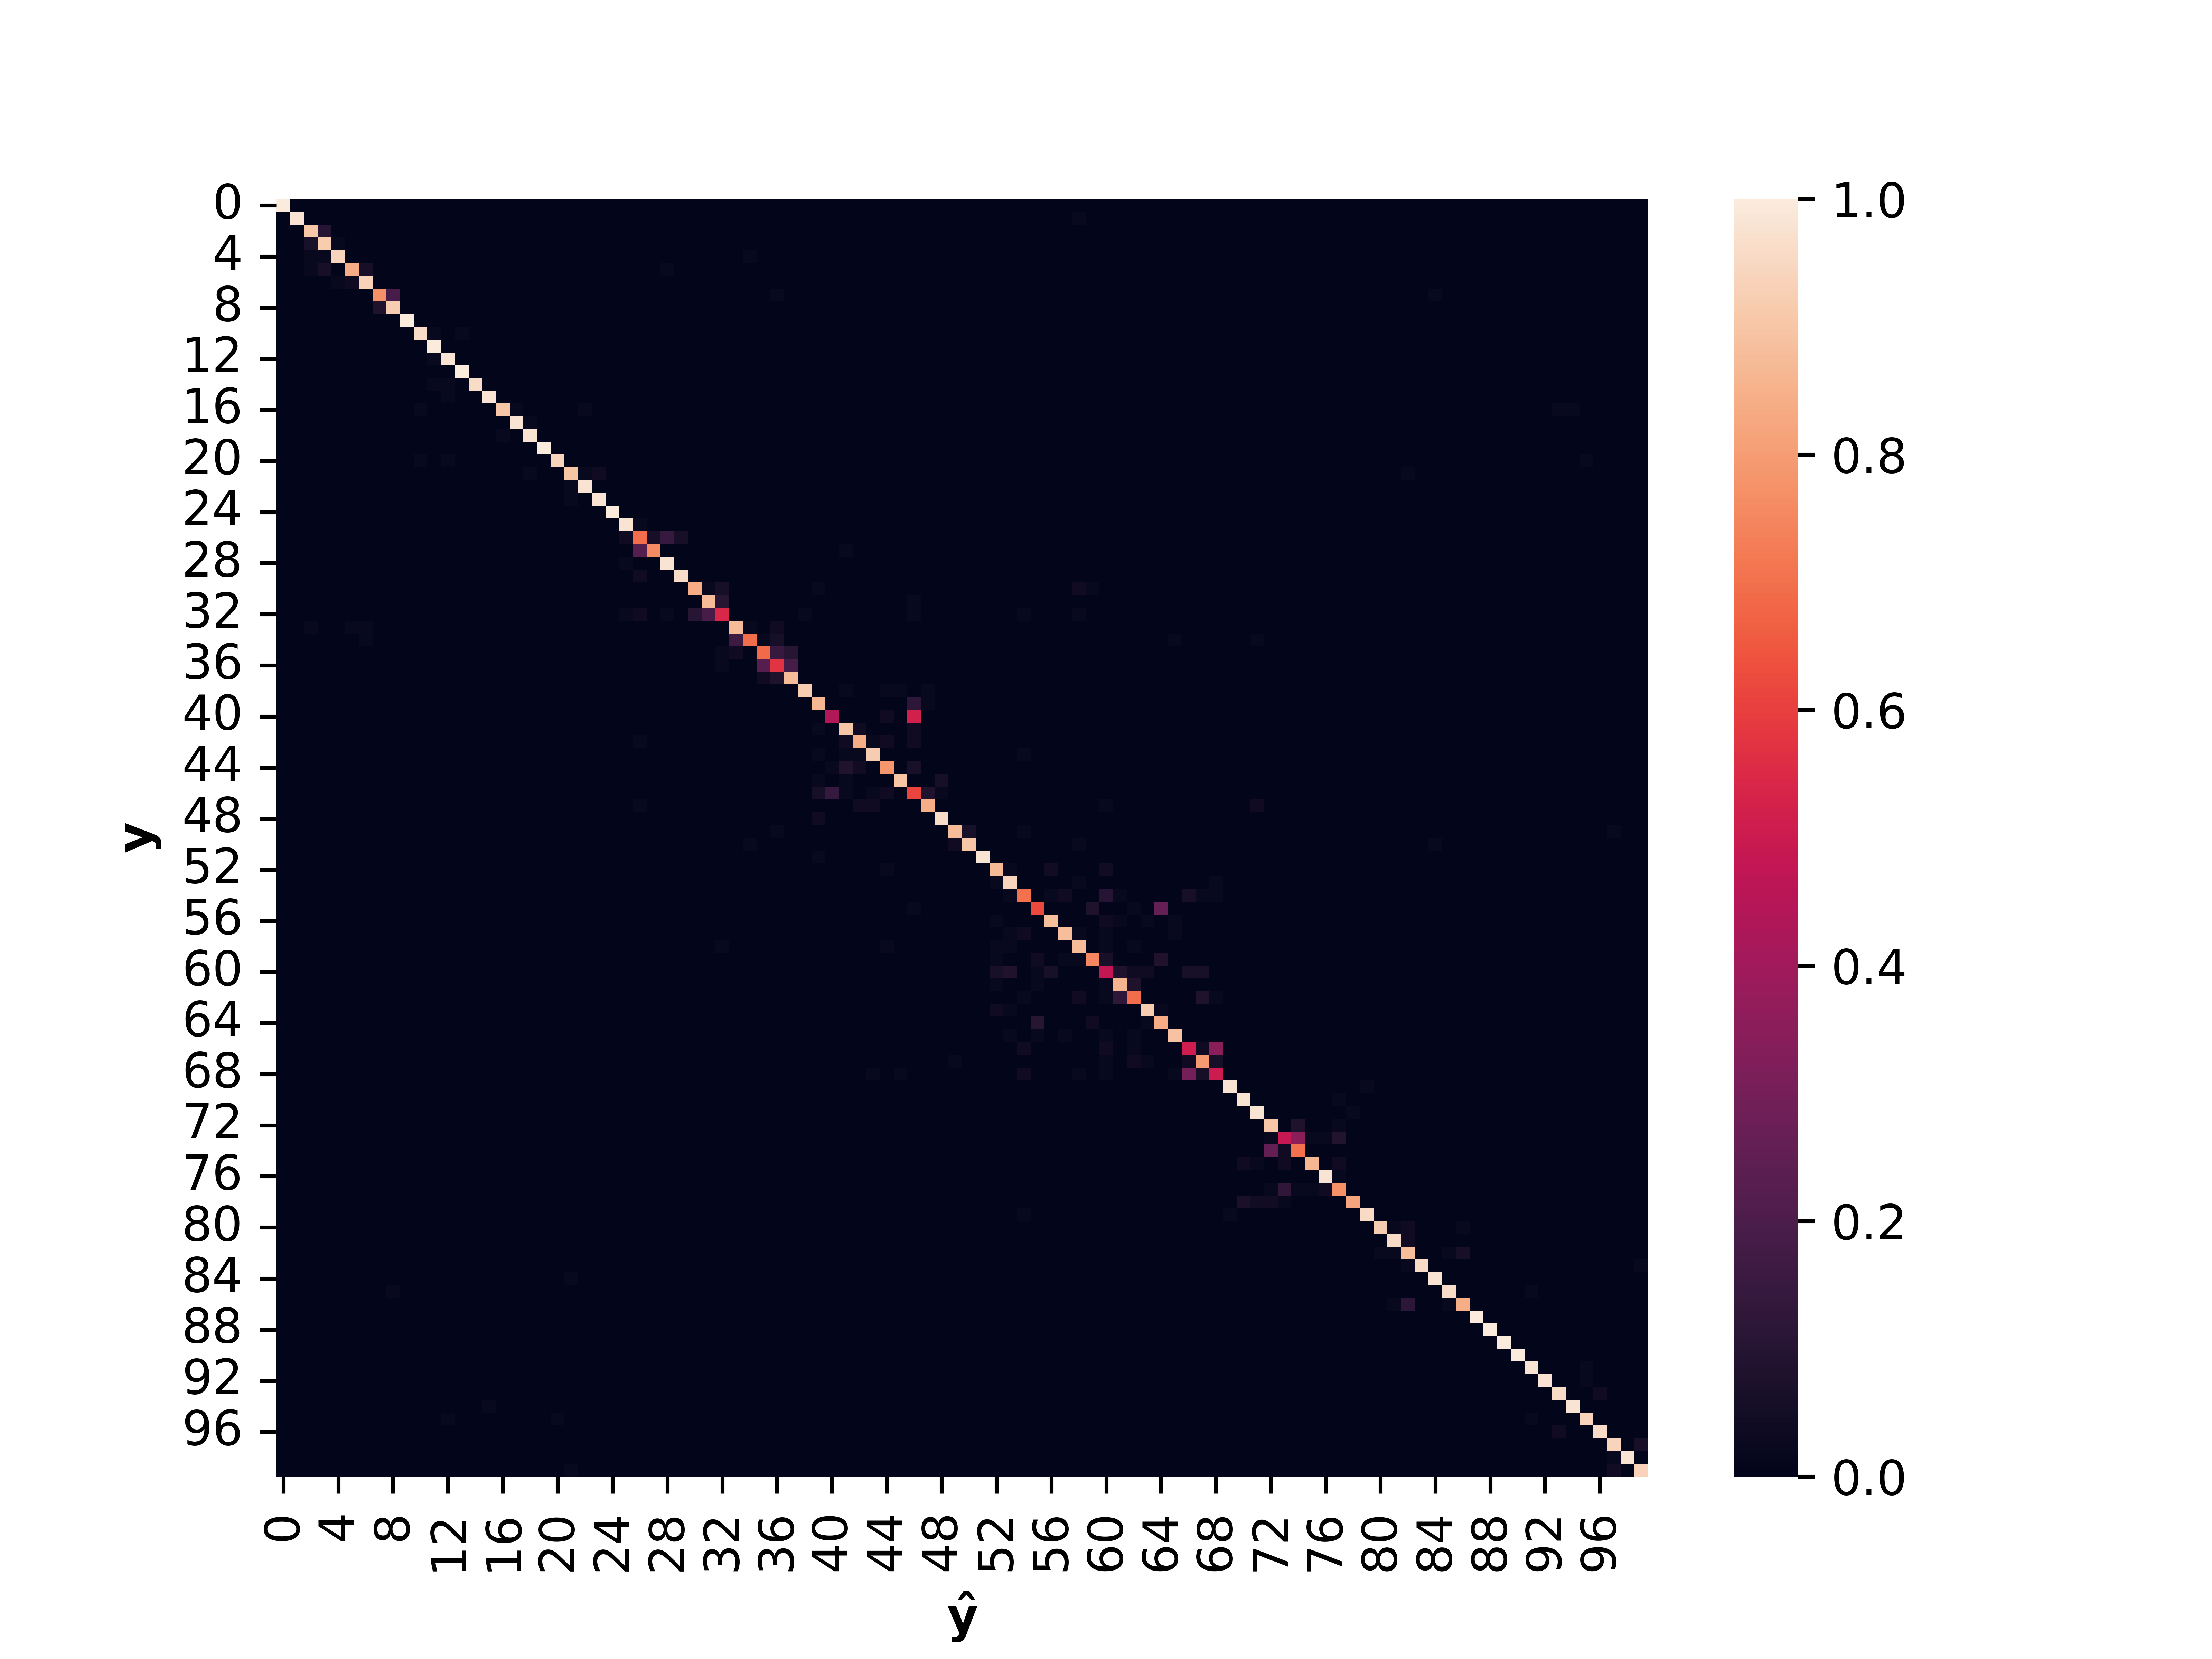
\includegraphics[height=0.4\textheight]{images/matrice_de_confusion_[0, 100].png}\label{subfig:confusion_matrix_a}}\hfill
  \subfigure[Matrice de confusion pour des labels compris entre 25 et 75]{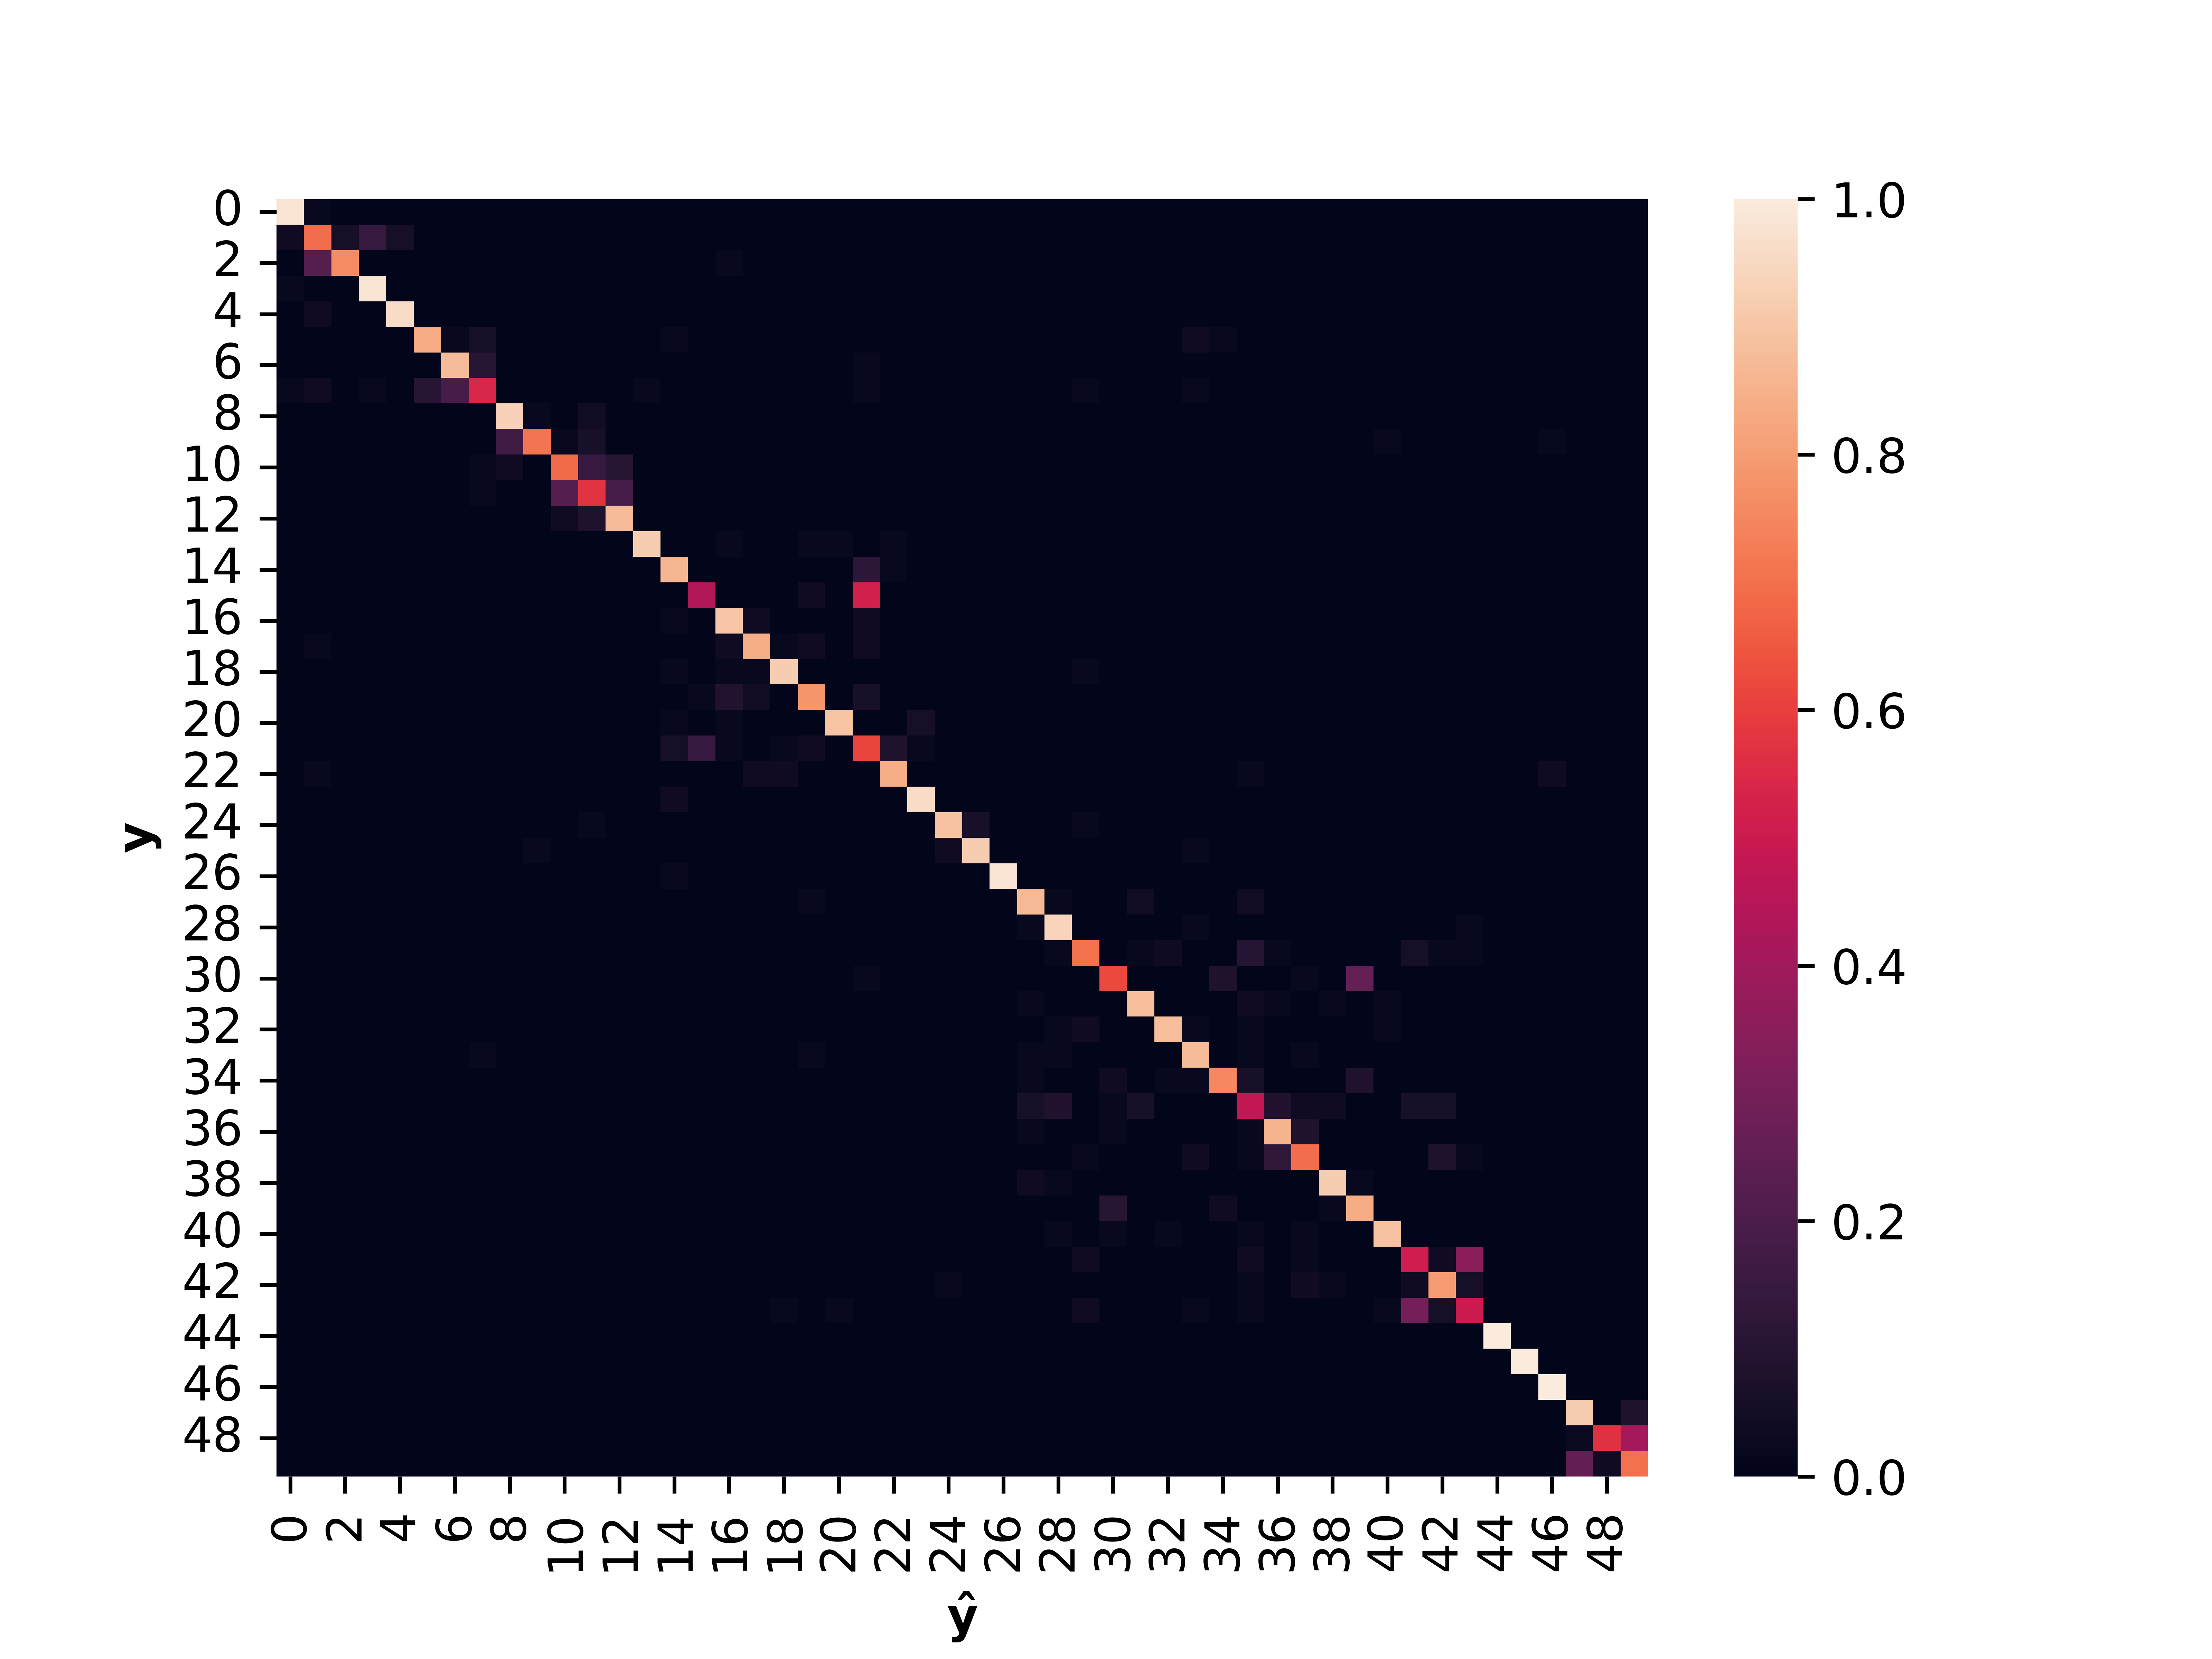
\includegraphics[height=0.4\textheight]{images/matrice_de_confusion_[25, 75].png}\label{subfig:confusion_matrix_b}}\hfill
  \caption{Représentation de la matrice de confusion associées à $\lambda = 10^{-4}$}
  \label{fig:confusion_matrix}
\end{figure}




Finalement, pour étudier les potentielles erreurs de classification liées à des similarités visuelles entre les classes, il faut s'intéresser à la construction de la base de donnée ImageNet. Comme introduit dans la section \ref{subsec:ImageNet}, ImageNet voit ses classes ordonnées selon l'architecture WordNet qui établit un lien sémantique entre les différentes classes. Ainsi, dans les ensembles de données d'ImageNet, les labels sont rangés par similitudes sémantiques au lieu d'être classés par ordre alphabétique par exemple. En traçant la matrice de confusion (figure \ref{fig:confusion_matrix}), on pourra ainsi détecter ces potentiels erreurs liés à cette proximité visuelle. Cependant, le nombre de classes étant important et le modèle suffisamment précis, il est difficile de réellement distinguer d'importantes confusions. En se concentrant sur de plus petites zones comme sur la figure \ref{subfig:confusion_matrix_b}, on distingue toutefois certains clusters d'erreur probablement dû à cette proximité visuelle inter-classes.

\chapter{Conclusion}
Dans cette étude, notre objectif initial était de former un modèle en explorant différentes valeurs de l'hyperparamètre de régularisation (le weight decay). Par la suite, nous avons cherché à identifier le meilleur modèle, c'est-à-dire le paramètre de weight decay optimal, pour résoudre notre problème d'optimisation global ainsi que les meilleures valeurs du weight decay pour la reconnaisance de chaque classe. Cette démarche s'est avérée cruciale car l'apprentissage des différentes classes se déroule à des rythmes disparates. Afin d'atténuer cet effet, nous avons appliqué une pénalisation sur l'apprentissage de nos modèles en ajustant le paramètre $\lambda$ de façon optimale.\\

Les valeurs du $\lambda$ optimal pour le problème d'optimisation globale ainsi que pour la reconnaissance de chaque classe ont été déterminées de plusieurs manières :\\

\begin{itemize}
    \item Taux de bonne classification en fonction des époques sur l'ensemble de test
    \item Fonction de coût en fonction des époques sur l'ensemble de test
    \item Fonction de coût en fonction de $\lambda$ sur l'ensemble de test
    \item Valeurs absolues des poids et des biais en fonction des époques
    \item La répartition des minimums des fonctions de coût pour chaque valeur de $\lambda$\\
\end{itemize}

A partir de ces valeurs de $\lambda$, nous avons pu représenter la fonction de coût associée à l'utilisation de l'optimisateur global du problème.

\chapter{Remerciements}

Finalement, ce projet de TX a été une occasion unique pour nous de nous former sur de multiples notions du deep learning, et plus particulièrement sur les réseaux de neurones convolutifs (CNN) et la régularisation dans le processus d'apprentissage.\\


Nous tenons à remercier tout particulièrement M. Yves Grandvalet pour son encadrement précieux et sa disponibilité tout au long de ce projet.

\bibliography{references.bib}



\end{document}
